\documentclass[12pt, titlepage]{article}

\usepackage{fullpage}
\usepackage[round]{natbib}
\usepackage{multirow}
\usepackage{booktabs}
\usepackage{tabularx}
\usepackage{graphicx}
\usepackage{float}
\usepackage{hyperref}
\hypersetup{
    colorlinks,
    citecolor=blue,
    filecolor=black,
    linkcolor=red,
    urlcolor=blue
}

%% Comments

\usepackage{color}

\newif\ifcomments\commentstrue %displays comments
%\newif\ifcomments\commentsfalse %so that comments do not display

\ifcomments
\newcommand{\authornote}[3]{\textcolor{#1}{[#3 ---#2]}}
\newcommand{\todo}[1]{\textcolor{red}{[TODO: #1]}}
\else
\newcommand{\authornote}[3]{}
\newcommand{\todo}[1]{}
\fi

\newcommand{\wss}[1]{\authornote{blue}{SS}{#1}} 
\newcommand{\plt}[1]{\authornote{magenta}{TPLT}{#1}} %For explanation of the template
\newcommand{\an}[1]{\authornote{cyan}{Author}{#1}}

%% Common Parts

\newcommand{\progname}{ProgName} % PUT YOUR PROGRAM NAME HERE
\newcommand{\authname}{Team \#, Team Name
\\ Student 1 name
\\ Student 2 name
\\ Student 3 name
\\ Student 4 name} % AUTHOR NAMES                  

\usepackage{hyperref}
    \hypersetup{colorlinks=true, linkcolor=blue, citecolor=blue, filecolor=blue,
                urlcolor=blue, unicode=false}
    \urlstyle{same}
                                


\newcounter{acnum}
\newcommand{\actheacnum}{AC\theacnum}
\newcommand{\acref}[1]{AC\ref{#1}}

\newcounter{ucnum}
\newcommand{\uctheucnum}{UC\theucnum}
\newcommand{\uref}[1]{UC\ref{#1}}

\newcounter{mnum}
\newcommand{\mthemnum}{M\themnum}
\newcommand{\mref}[1]{M\ref{#1}}

\begin{document}

\title{System Design for \progname{}} 
\author{\authname}
\date{\today}

\maketitle

\pagenumbering{roman}

\section{Revision History}

\begin{tabularx}{\textwidth}{p{3cm}p{2cm}X}
\toprule {\bf Date} & {\bf Version} & {\bf Notes}\\
\midrule
01/13/2024 & 0.0 & Initial draft of all sections\\
01/15/2024 & 0.1 & Edits to the component diagram and the connections\\
01/17/2024 & 0.2 & Final edits and check for grammar and clarity \\
\bottomrule
\end{tabularx}

\newpage

\section{Reference Material}

This section records information for easy reference.

\subsection{Abbreviations and Acronyms}
\renewcommand{\arraystretch}{1.2}
\begin{tabular}{l l} 
    \toprule		
    \textbf{symbol} & \textbf{description}\\
    \midrule 
    \progname & Explanation of program name\\
    AUC & Area Under Curve\\
    \multirow{3}{*}{DICOM} & Digital Imaging and Communications in Medicine; \\ & technical standard for digital storage/transmission \\ & of medical images and related information \\
     \multirow{2}{*}{JPEG/JPG} & Joint Photographic Experts Group; \\ & digital image compression standard, image format \\
    M & Module \\
    MG & Module Guide \\
    MIS & Module Interface Specification \\ 
    MVC & Model-View-Controller Software Architecture \\
    NLP & Natural Language Processing \\
    R & Requirement \\
    \multirow{3}{*}{ROC curve} & Receiver Operating Characteristic curve, \\ & a graph to show the performance of a model,\\ & plots true positive
    rate and false positive rate\\
    SRS & Software Requirement Specification \\
    \multirow{3}{*}{\progname} & The Process of Designing and Developing Software; \\
    & a reference to the software application described \\
    & in this document \\
    \bottomrule
\end{tabular}\\
% \caption{Symbols, Abbreviations and Acronyms}
% \label{table:SysAbbreviations&Acronyms}


\newpage

\tableofcontents

\newpage

\listoftables

\listoffigures

\newpage

\pagenumbering{arabic}

\section{Introduction}
This document aims to outline the system design that meets the requirements defined in the project SRS (SRS Section 2).
It will cover the general system with more details about the software architecture outlined in the MG document, and the detailed module interface specification in the MIS document.

\section{Purpose}
The purpose of this document is to communicate the overall system design. This document focuses on outlining how the system interacts with its environment, the expected operation and unexpected event handling, the explicit relation between design decisions and the requirements seen in the SRS (SRS Section 2), how the system is divided into components, user interface, and the timeline and any constraints for the project.

The purpose of the system is to aid medical professionals and specifically radiologists by reducing the amount of time they need to spend reviewing chest X-rays of patients by conducting a preliminary scan on a patient x-ray for four diseases, Atelectasis, Cardiomegaly, Pleural Effusion, and Pneumonia, with a greater AUC of the ROC than existing systems to create a higher level of confidence in the systems correct predictions. 

\section{Scope}
The system is designed for use by medical professionals at hospitals, labs and offices to conduct a preliminary scan of a patient's chest X-ray and highlight the risk of four diseases identifiable from chest X-rays. 

The diagram below outlines where our system interacts with the surrounding environment and the boundaries of our system. 
\begin{figure}[H]
    \centering
    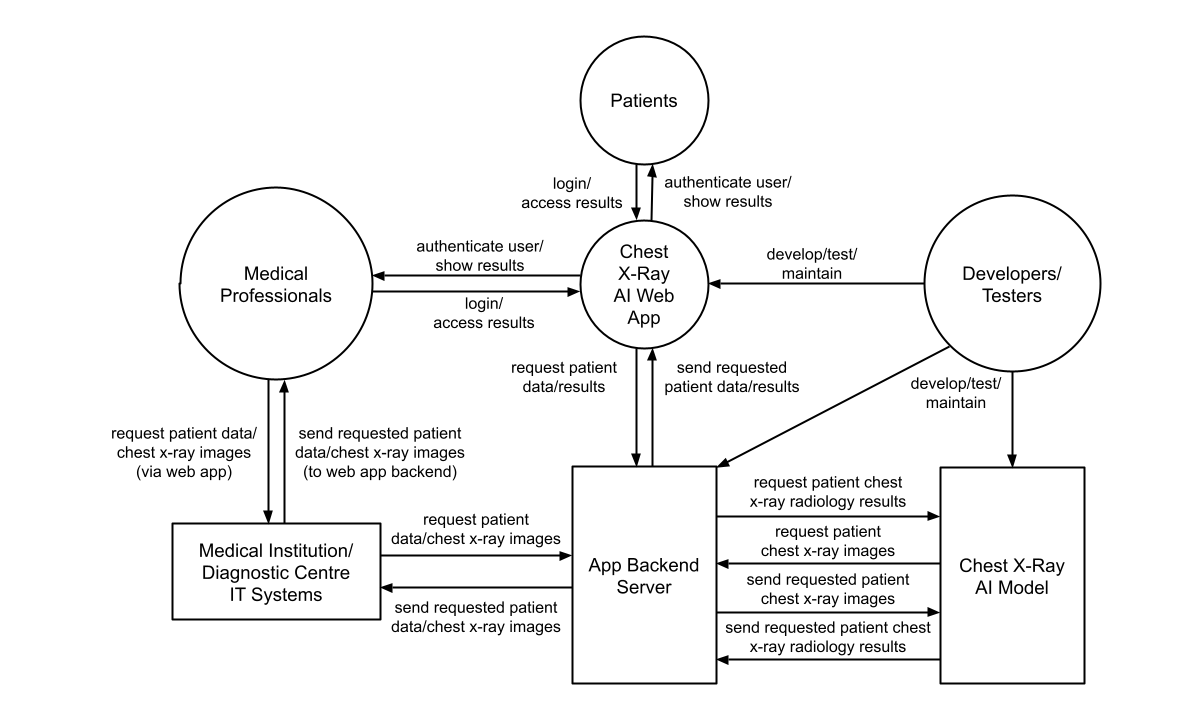
\includegraphics[scale=0.25]{Context Diagram for Chest X-Ray AI Read.png}
    \caption{Context Diagram describing The Context of the Work}
    \label{fig:contextDiagram}
\end{figure}

\section{Project Overview}
\subsection{Normal Behaviour}
The system is to be used through a web-application that requires a computer and stable access to the internet. This allows for the system to be used within any existing enterprise systems within hospitals, offices, and labs without the need to understand and integrate into each individual use.
\begin{enumerate}
    \item \bf{Chest X-Ray Read Module}: Reads the JPEG of the X-ray, after conversion from DICOM.
    \item \bf{Results Generation Module}: Generates a disease risk classification for the X-ray input.
    \item \bf{Report Component Generation Module}: Generates a brief diagnosis report for the X-ray input.
    \item \bf{Database Operations Module}: Contains database management functions for the patient database.
    \item \bf{User Authentication/Management Module}: Responsible for authorizing user login credentials.
    \item \bf{App GUI Module}: The graphical user interface of the system.
    \item \bf{Login Module}: Login page UI view.
    \item \bf{Perform Scan Module}: UI view for submitting X-ray input to the system to perform a diagnosis.
    \item \bf{View Results Module}: View for the results of the scan and disease report.
    \item \bf{AI Model Module}: AI model for identifying diseases in the X-ray input.
    \item \bf{NLP Model Module}: Model for generating a breif diagnosis report using NLP.
    \item \bf{Backend Module}: Module that interfaces with DICOM server containing patient data.
    \item \bf{App Controller Module}: Controller for interacting with the different models and views.
    \item \bf{Medical Institution Interface Module}: Allows information upload, for DICOM files, between application and the medical institutions' IT system.
\end{enumerate}

\subsection{Undesired Event Handling}
The system handles undesired events, such as incorrect data, by first checking that any alterations to the data or system will not result in an unsafe state. Should the system receive improper data or experience a connection issue it will prevent further operation until the issue has deemed resolved by the system. The user will need to recommence their actions from login in order to prevent storage of incorrect data. 

\subsection{Component Diagram}
\begin{figure}[H]
    \centering
    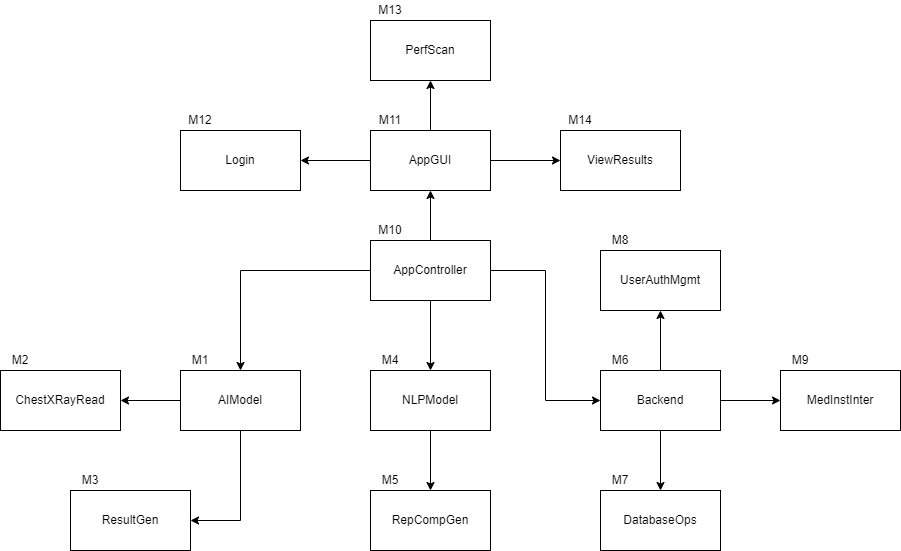
\includegraphics[scale=0.55]{UsesHierarchy.png}
    \caption{Component Diagram that shows the interaction of components}
    \label{fig:componentDiagram}
\end{figure}

\subsection{Connection Between Requirements and Design} \label{SecConnection}
The design of the system is intended to satisfy the requirements developed in
the SRS. 
\begin{enumerate}
    \item FR4: We decided that the best way to display a structured set of data about a patient was to display all findings in table format.
    \item FR11: To allow for multiple different key searches we decided to have one search entry field but allow the user to select an option on what data is used in the search. (ie. ID or name) 
    \item NFAR0: Our choice for 'clean' design meant minimal colour changes and minimal feature other than those necessary. 
    \item NFLR0: The system follows similar design to other systems already used in medical offices/hospitals, so there is minimal learning required for operation. 
    \item NFSR0: A description of the main features and functionality of the system will be available on the main page.
    \item NFAR0: Users will require a username and password to verify authorization to patient data. 
\end{enumerate}

\section{System Variables}
\subsection{Monitored Variables}
N/A

\subsection{Controlled Variables}
N/A

\subsection{Constants Variables}
N/A

\section{User Interfaces}
Our system only has a software component for user interaction, and in following the non-functional requirements defined in SRS sections 3.1 and 3.2, uses a simple, consistent colour theme and only the necessary elements for operation. It also follows common design principles and patterns to be conducive to intuitive understanding and quick comprehension of the system.
The \hyperlink{A}{appendix} contains all the current web page designs. 

\section{Timeline}
\begin{table}
    \begin{tabular}{l l l} 
    \toprule		
    \textbf{Deliverable} & \textbf{Assigned to} & \textbf{Deadline}\\
    \midrule 
    \textbf{Model Module} & \\
    \midrule
    ChestXRayread & Tushar, Mohaansh, Ibrahim & January 21, 2024 \\
    ResultsGen & Ibrahim & January 21, 2024\\
    ResCompgen & Tushar & January 21, 2024\\
    DatabaseOps & Nathaniel & January 22, 2024\\
    UserAuthMgmt & Nathaniel & January 22, 2024\\
    MedInstInter & Allison & January 21, 2024 \\
    \midrule
    \textbf{View Module} \\
    \midrule
    Login & Allison & January 24, 202 \\
    PerfScan & Allison & January 24, 202\\
    ViewResults & Allison & January 24, 2024 \\
    \midrule
    \textbf{Controller Module} \\
    \midrule
    AIModel & Tushar, Mohaansh, Ibrahim & January 20, 2024\\
    NLPModel & Allison & February 1, 2024\\
    Backend & Nathaniel & January 21, 2024\\
    AppController & Nathaniel & January 21, 2024\\
    AppGUI & Allison & January 21, 2024\\
    \midrule
    \textbf{Testing} \\
    \midrule
    Model Module & Mohaansh with participants & February 3, 2024 \\
    View Module review & Allison with participants & January 26, 2024 \\
    Controller Module & Allison, Nathaniel & February 2, 2024  \\
    System & Allison, Ibrahim, Mohaansh, Nathaniel, Tushar & February 5, 2024 \\
    \bottomrule
    \end{tabular}\\
    \caption{Implementation Timeline}
    \label{table:Timeline}
\end{table}

% \bibliographystyle {plainnat}
% \bibliography{../../../refs/References}

\newpage{}

\appendix

\section{Interface}
\hypertarget{A}{The} interface appendix includes all Figma images that illustrate the design of the user interface. 

\begin{figure}[H]
    \centering
    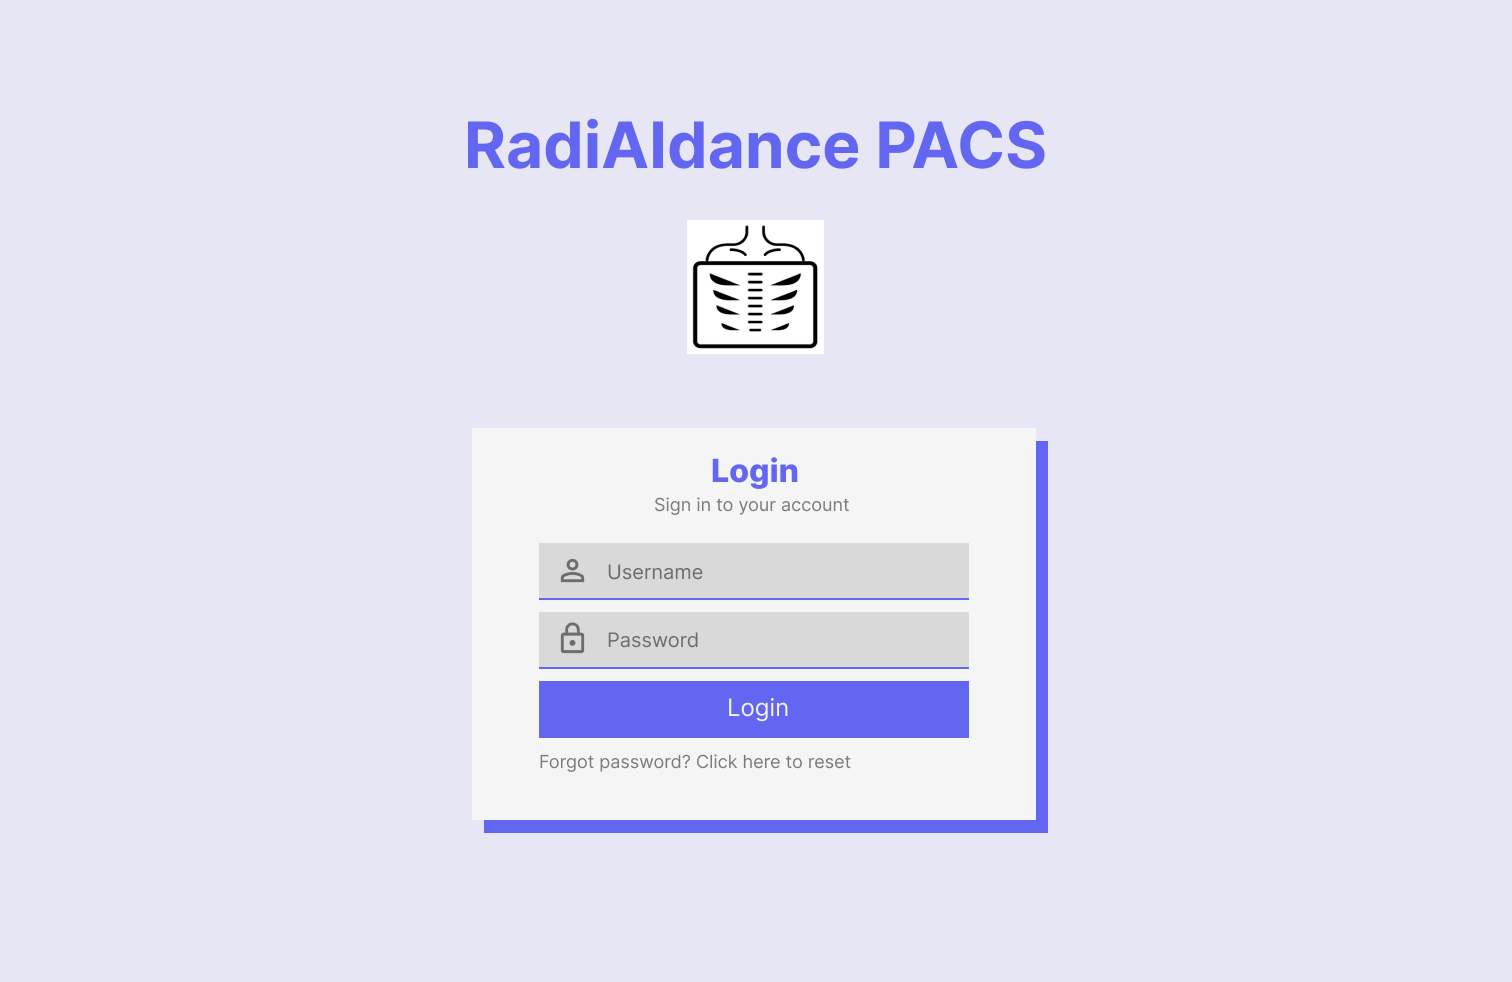
\includegraphics[scale=0.30]{chest-x-ray-ai.png}
    \caption{Login page, the first page seen by users}
    \label{fig:LoginPage}
\end{figure}
\begin{figure}[H]
    \centering
    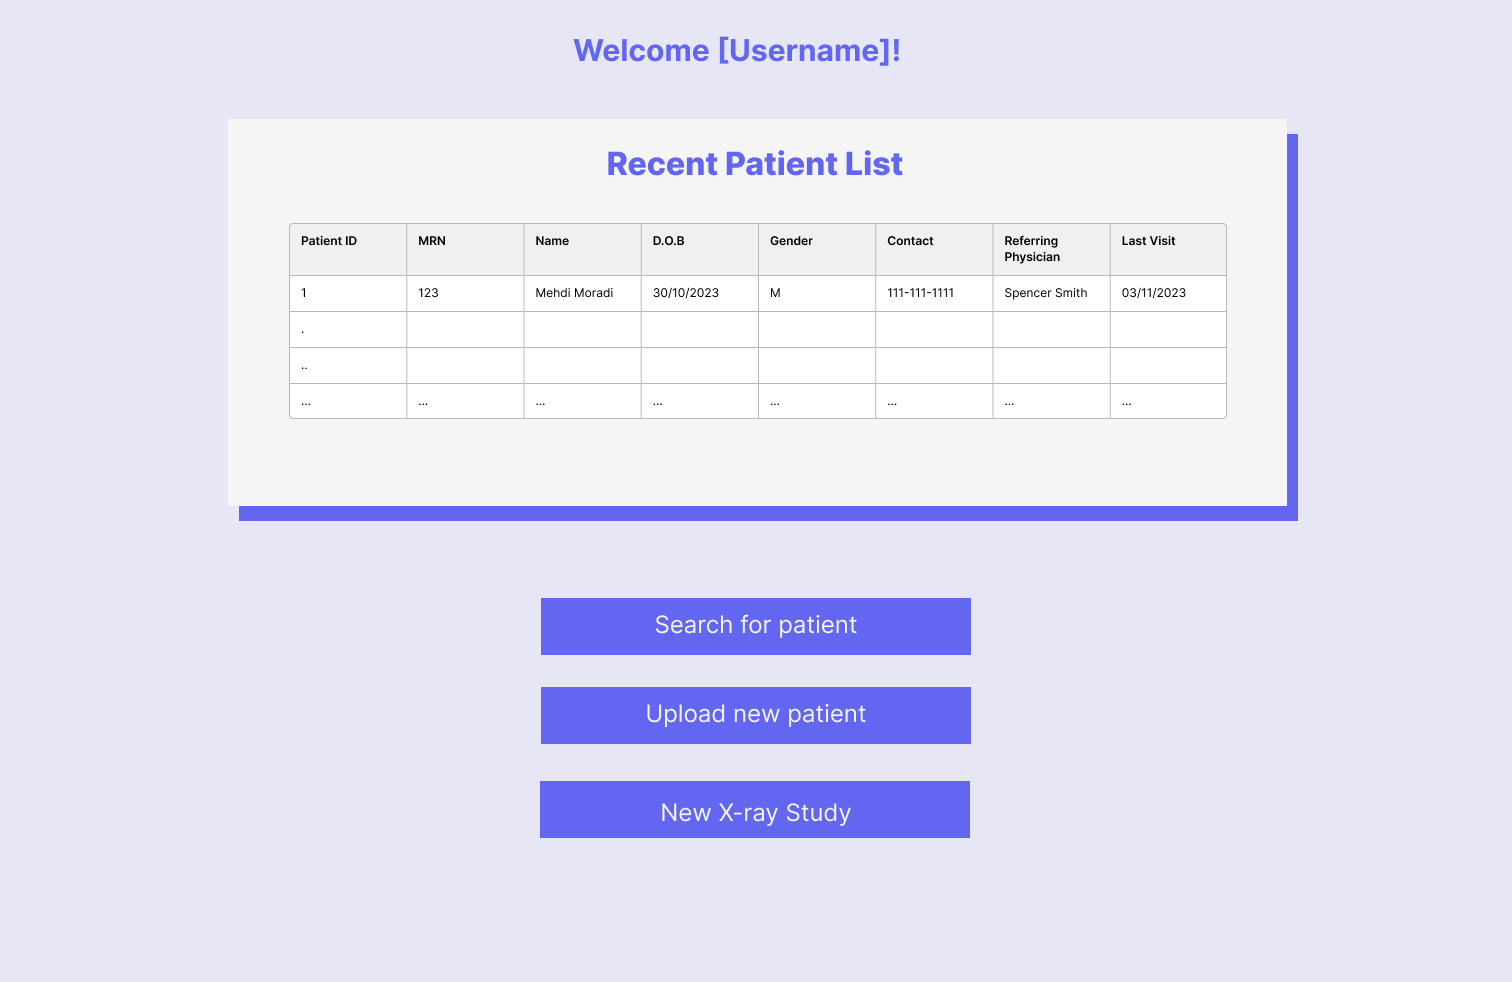
\includegraphics[scale=0.30]{chest-x-ray-ai (6).png}
    \caption{Main page with all main functions}
    \label{fig:MainPage}
\end{figure}
\begin{figure}[H]
    \centering
    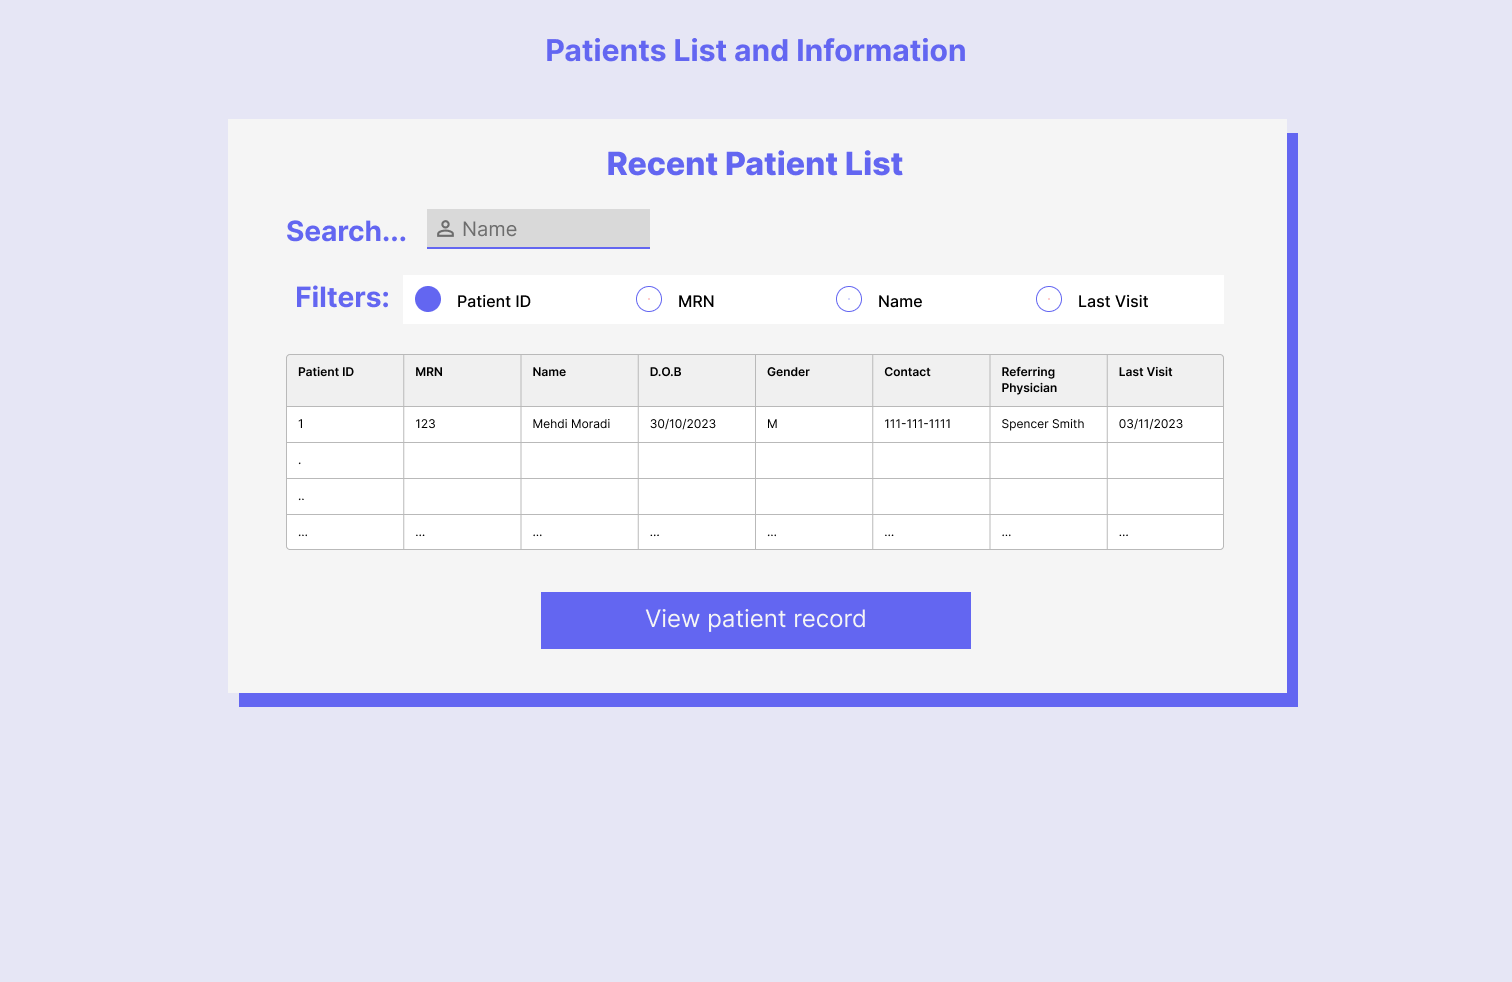
\includegraphics[scale=0.30]{chest-x-ray-ai (2).png}
    \caption{Search page used to search through all existing patient records}
    \label{fig:PatientSearchPage}
\end{figure}
\begin{figure}[H]
    \centering
    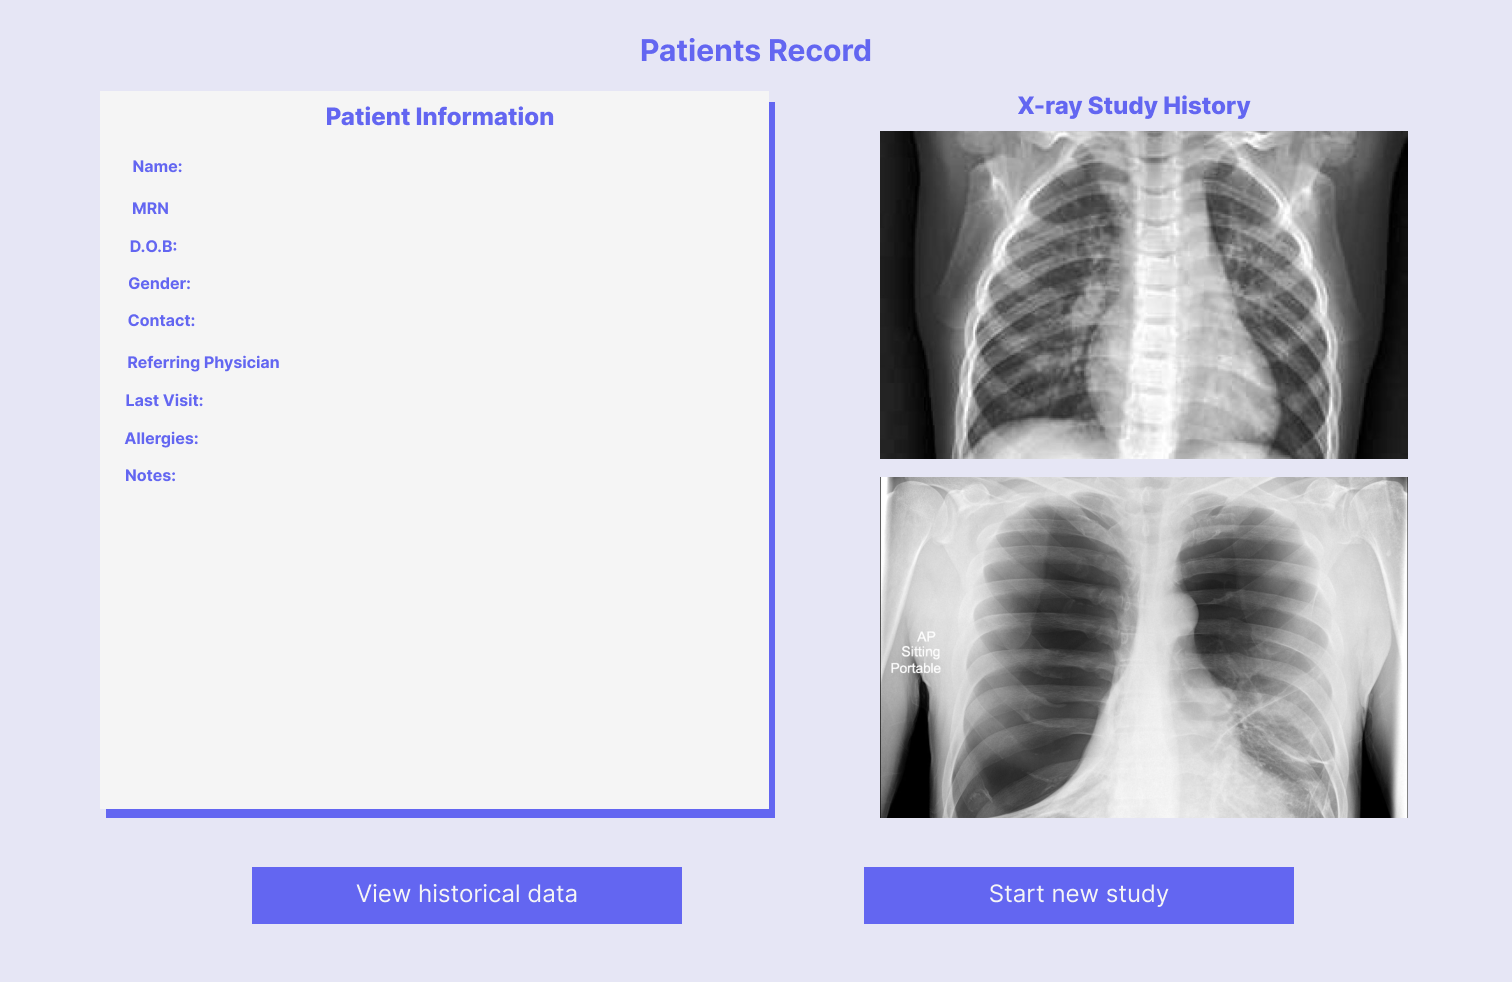
\includegraphics[scale=0.30]{chest-x-ray-ai (3).png}
    \caption{Page that displays a selected patients records}
    \label{fig:PatientRecordPage}
\end{figure}
\begin{figure}[H]
    \centering
    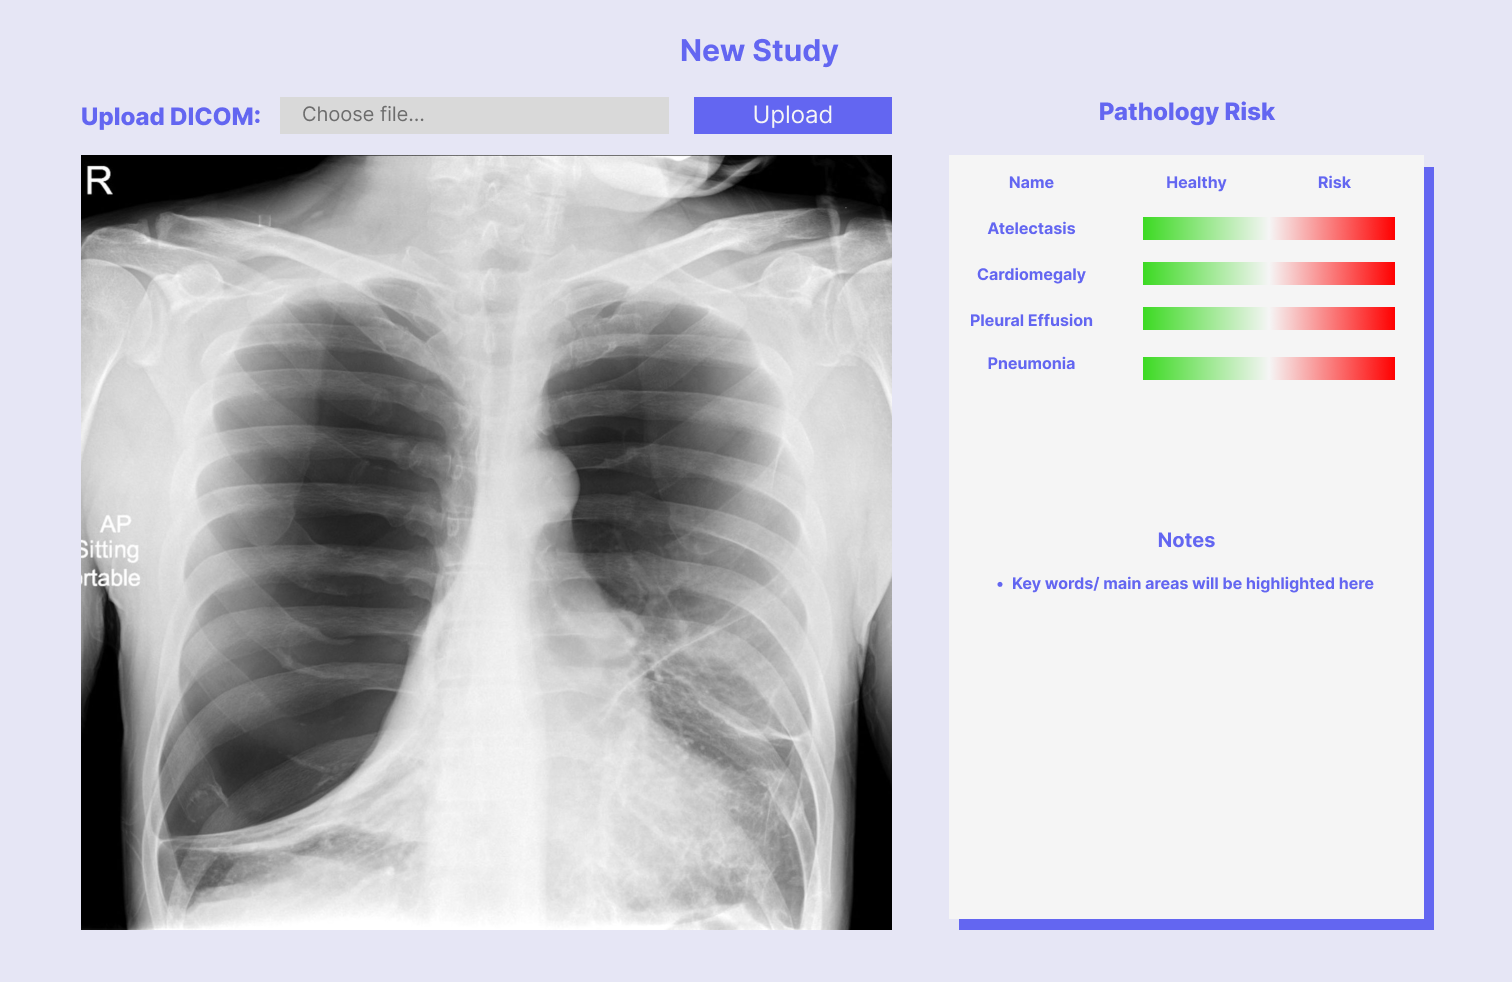
\includegraphics[scale=0.30]{chest-x-ray-ai (4).png}
    \caption{Page which displays the results of a new chest-x-ray uploaded to the system}
    \label{fig:NewStudeyPage}
\end{figure}
\begin{figure}[H]
    \centering
    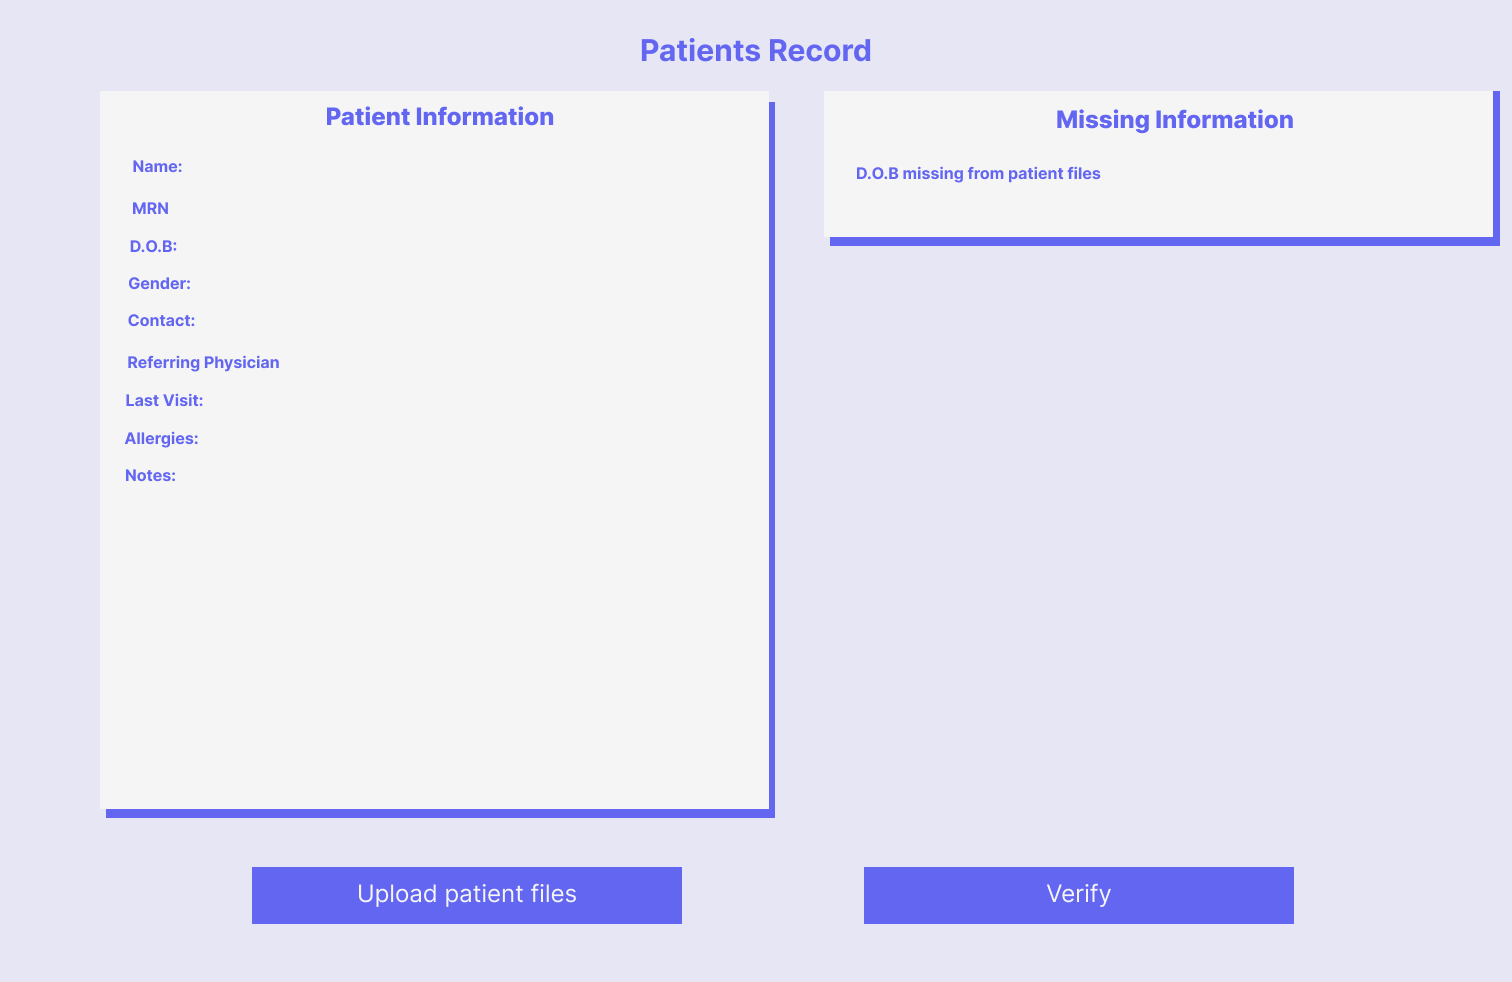
\includegraphics[scale=0.30]{chest-x-ray-ai (5).png}
    \caption{The page that allows new patients to be added to the system before conducting a new chest-x-ray review}
    \label{fig:NewPaitentRecordPage}
\end{figure}


\section{Reflection}
\begin{enumerate}
    \item Some limitations of the solution is the number of diseases, we are focusing on improving the AUC of the ROC for only 4 diseases, with more time, computational power, access to better dataset and/or additional time to conduct our own data creation with material professional (doctors \& radiologists), we could aim to improve the AUC of ROC for more diseases, allowing the solution to give more time to the limited doctors to be able to save more people and improve the medical system.
    \item Some other design solutions we considered were making the application as a local desktop app. Instead, the data is stored on a cloud based system (web app).
    \item The alternate design choice of making a desktop application would pose storage limitations, and there would need to be special considerations for device and system specifications (e.g. development for macOS, windows, etc.), The software was chosen to be a web app because it would be easier to use a cloud service to store data, and web pages are a more universal and easier to maintain interface. A trade-off for this is that specific data security protocols would need to be implemented as it is not local.
\end{enumerate}

\end{document}